\documentclass[12pt]{article}
\usepackage[utf8]{inputenc}
\usepackage[spanish,es-lcroman, es-tabla]{babel}
\usepackage[autostyle,spanish=mexican]{csquotes}
\usepackage{amsmath}
\usepackage{amssymb}
\usepackage{nccmath}
\numberwithin{equation}{section}
\usepackage{amsthm}
\usepackage{graphicx}
\usepackage{epstopdf}
\DeclareGraphicsExtensions{.pdf,.png,.jpg,.eps}
\usepackage{color}
\usepackage{float}
\usepackage{multicol}
\usepackage{enumerate}
\usepackage[shortlabels]{enumitem}
\usepackage{anyfontsize}
\usepackage{anysize}
\usepackage{array}
\usepackage{multirow}
\usepackage{enumitem}
\usepackage{cancel}
\usepackage{tikz}
\usepackage{circuitikz}
\usepackage{tikz-3dplot}
\usetikzlibrary{babel}
\usetikzlibrary{shapes}
\usepackage{bm}
\usepackage{mathtools}
\usepackage{esvect}
\usepackage{hyperref}
\usepackage{relsize}
\usepackage{siunitx}
\usepackage{physics}
%\usepackage{biblatex}
\usepackage{standalone}
\usepackage{mathrsfs}
\usepackage{bigints}
\usepackage{bookmark}
\spanishdecimal{.}

\setlist[enumerate]{itemsep=0mm}

\renewcommand{\baselinestretch}{1.5}

\let\oldbibliography\thebibliography

\renewcommand{\thebibliography}[1]{\oldbibliography{#1}

\setlength{\itemsep}{0pt}}
%\marginsize{1.5cm}{1.5cm}{2cm}{2cm}


\newtheorem{defi}{{\it Definición}}[section]
\newtheorem{teo}{{\it Teorema}}[section]
\newtheorem{ejemplo}{{\it Ejemplo}}[section]
\newtheorem{propiedad}{{\it Propiedad}}[section]
\newtheorem{lema}{{\it Lema}}[section]

\marginsize{1.5cm}{1.5cm}{2cm}{2cm} 
\title{Sistemas de coordenadas curvilíneas ortogonales \\ {\large Matemáticas Avanzadas de la Física}}
\date{ }
\begin{document}
\renewcommand\labelenumii{\theenumi.{\arabic{enumii}}}
\maketitle
\fontsize{14}{14}\selectfont
\vspace{-2cm}
%Referencia: Happel - Low Reynolds number hydrodynamics - Appendix A
\section{Coordenadas curvilíneas.}
La posición de un punto en el espacio tridimensional (con respecto a algún origen) generalmente se especifica al dar sus tres coordenadas cartesianas $(x, y, z)$ o, lo que es equivalente, al especificar el vector de posición $\vb{R}$ del punto. A menudo es más conveniente describir la posición del punto por otro conjunto de coordenadas más apropiadas para el problema en cuestión, los ejemplos comunes son coordenadas esféricas y cilíndricas. Estos son solo casos especiales de \emph{sistemas de coordenadas curvilíneas}, cuyas propiedades generales proponemos examinar en detalle.
\par
Supongamos que $q_{1}, q_{2}, q_{3}$ son funciones independientes de la posición, tales que
\begin{align}
q_{1} = q_{1} (x, y, z), \hspace{1cm} q_{2} = q_{2} (x, y, z), \hspace{1cm} q_{3} = q_{3} (x, y, z)
\label{eq:ecuacion_A_01_01}
\end{align}
o en términos de un vector de posición
\begin{align*}
q_{k} = q_{k}(\vb{R}) \hspace{1cm} k = 1, 2, 3
\end{align*}
En las regiones donde el determinante Jacobiano
\begin{align}
\pdv{(q_{1}, q_{2}, q_{3})}{(x, y, z)} = 
\mdet{\displaystyle \pdv{q_{1}}{x} & \displaystyle \pdv{q_{1}}{y} & \displaystyle \pdv{q_{1}}{z} \\[1em]
\displaystyle \pdv{q_{2}}{x} & \displaystyle \pdv{q_{2}}{y} & \displaystyle \pdv{q_{2}}{z} \\[1em]
\displaystyle \pdv{q_{3}}{x} & \displaystyle \pdv{q_{3}}{y} & \displaystyle \pdv{q_{3}}{z} \\
}
\label{eq:ecuacion_A_01_02}
\end{align}
es diferente de cero, este sistema de ecuaciones se puede resolver simultáneamente para $x, y, z$, obteniendo
\begin{align}
x = x (q_{1}, q_{2}, q_ {3}) \hspace{1cm} y = y (q_{1}, q_{2}, q_ {3}) \hspace{1cm} z = z (q_{1}, q_{2}, q_ {3})
\label{eq:ecuacion_A_01_03}    
\end{align}
o en términos de un vector
\begin{align*}
\vb{R} = \vb{R} (q_{1}, q_{2}, q_{3})
\end{align*}
Que el Jacobiano se anule implica que $q_{1}, q_{2}$ y $q_{3}$ son funciones no independientes, sino que están conectadas por una relación funcional de la forma $f (q_{1}, q_{2}, q_{3}) = O$.
\par
De acuerdo con la ec.(\ref{eq:eq:ecuacion_A_01_03}), asignarle valores numéricos para $q_{1}, q_{2}$ y $q_{3}$ conduce a un conjunto correspondiente de valores numéricos para $x, y, z$; es decir, localiza un punto $(x, y, z)$ en el espacio. De este modo, llegamos a considerar el conjunto de tres números $(q_{1}, q_{2}, q_{3})$ como las \emph{coordenadas curvilíneas} de un punto en el espacio. Es natural al tratar problemas físicos restringir la atención a los sistemas de coordenadas curvilíneas en los que cada punto en el espacio puede representarse al menos una vez dejando que $q_{1}, q_{2}$ y $q_{3}$ varíen sobre todos los valores posibles.
\par
Las coordenadas curvilíneas tienen una interpretación geométrica simple. Si por el momento asignamos algún valor constante a $q_{k}$ tenemos
\begin{align*}
q_{k} (x, y, z) = \mbox{ constante} \hspace{0.5cm} (k = 1, 2, 3)
\end{align*}
 que describe una superficie en el espacio. Al asignar una serie de valores diferentes a $q_{k}$, generamos una \emph{familia de superficies} en las que $q_{k}$ es constante. Si las funciones se han elegido correctamente, hay al menos una superficie que pertenece a cada una de las tres familias que pasa por cualquier punto arbitrario $P$ en el espacio. Por lo tanto, un punto en el espacio se caracteriza por la intersección de las tres superficies, $q_{1} = \mbox{ constante}, q_{2} = \mbox{ constante}, q_{3} = \mbox{ constante}$ (ver la figura \ref{fig:figura_A_01}), denominadas \emph{superficies coordenadas}. La superficie coordenada se llama para esa coordenada que es constante, las otras dos coordenadas son variables a lo largo de esa superficie
\begin{figure}[H]
    \centering
    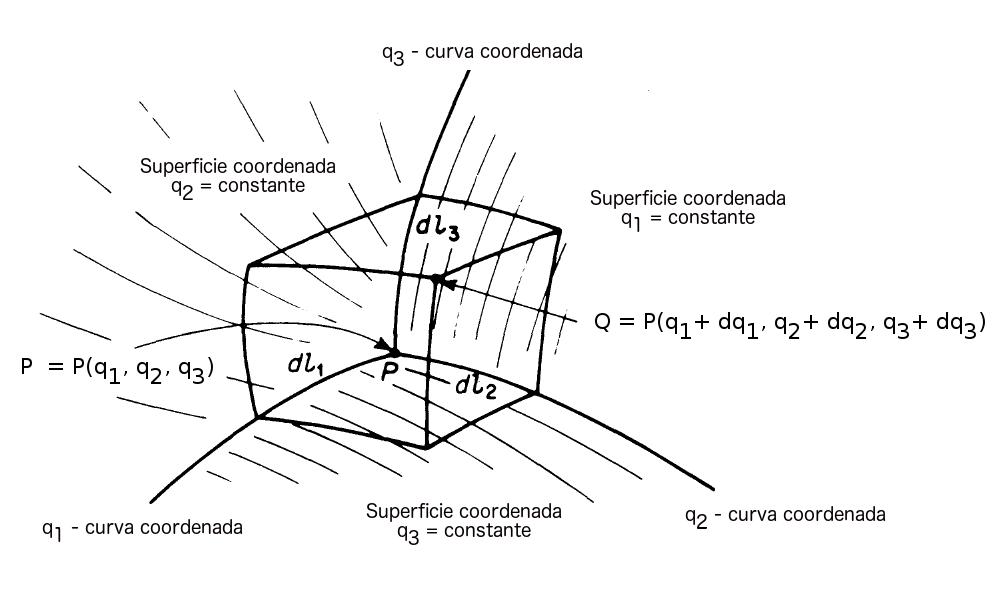
\includegraphics[scale=0.35]{Imagenes/CoordenadasCurvilineas_01.png}
    \caption{Sistema de coordenadas curvilíneas.}
    \label{fig:figura_A_01}
\end{figure}
La intersección de dos superficies coordenadas da como resultado una curva sesgada denominada \emph{curva de coordenadas}. Por ejemplo, la intersección de las superficies coordenadas $q_{2}$ y $q_{3}$ da como resultado la curva de coordenadas etiquetada $q_{1}$.
\par
Como esta curva se encuentra simultáneamente en las superficies $q_{2}$ = constante y $q_{3}$ = constante, solo $q_{1}$ varía a medida que avanzamos a lo largo de la curva; de ahí, que se le llame curva de coordenada $q_{1}$.
\par
En el caso especial de coordenadas cartesianas, las superficies coordenadas constan de tres planos mutuamente perpendiculares; las curvas coordenadas consisten en tres líneas perpendiculares entre sí.
\par
En coordenadas cartesianas, los diferenciales $\dd{x}, \dd{y}, \dd{z}$ corresponden a distancias medidas a lo largo de cada una de las tres curvas de coordenadas cartesianas. Los diferenciales análogos en coordenadas curvilíneas, $\dd{q_{1}}, \dd{q_{2}}, \dd{q_{3}}$, no tienen necesariamente una interpretación similar. Como en la figura \ref{fig:figura_A_01}, sea $\dd{l_{1}}$ la distancia medida a lo largo de la curva $q_{1}-$coordenada desde el punto $P (q_{1}, q_{2}, q_{3})$ al punto vecino $(q_{1} + \dd{q_{1}}, q_{2}, q_{3})$. Se aplica la misma definición para $\dd{l_{2}}$ y $\dd{l_{3}}$. Definimos las tres cantidades.
\begin{align}
h_{k} =  \abs{\dv{q_{k}}{l_{k}}} > 0, \hspace{1cm} k = 1, 2, 3
\label{eq:ecuacion_A_01_04}    
\end{align}
Esas cantidades (o variantes de ellas) se llaman \emph{coeficientes métricos}. Son propiedades intrínsecas de cualquier sistema particular de coordenadas curvilíneas y, en general, son funciones de posición,
\begin{align*}
h_{k} = k_{k} (q_{1}, q_{2}, q_{3})
\end{align*}
Sean $\vu{i}_{1}, \vu{i}_{2}$ y $\vu{i}_{3}$ los vectores unitarios que son tangentes a las curvas de coordenadas $q_{1}$, $q_{2}$, $q_{3}$ respectivamente, en las direcciones en las que $q_{k}$ algebraicamente se incrementan, ver la figura \ref{fig:figura_A_02}.
\begin{figure}[H]
    \centering
    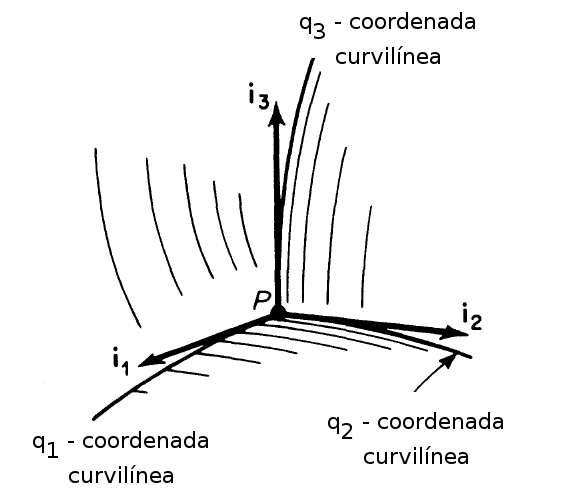
\includegraphics[scale=0.4]{Imagenes/CoordenadasCurvilineas_02.png}
    \caption{Vectores unitarios tangentes.}
    \label{fig:figura_A_02}
\end{figure}
Es evidente que esos vectores unitarios tangentes están dados por
\begin{align}
\vu{i}_{k} = \pdv{\vb{R}}{l_{k}} \hspace{1cm} k = 1, 2, 3
\label{eq:ecuacion_A_01_05}    
\end{align}
Mientras que las \emph{magnitudes} de estos vectores unitarios son necesariamente constantes
\begin{align}
\vu{i}_{k} \cdot \vu{i}_{k} =  1 \hspace{1cm} \mbox{o} \hspace{1cm} \abs{\vu{i}_{k}} = 1
\label{eq:ecuacion_A_01_06}
\end{align}
no se sigue que sus \emph{direcciones} permanezcan constantes de un punto a otro, por lo que los vectores unitarios son, en general, funciones de posición
\begin{align*}
\vu{k} = \vu{i}_{k} (q_{1}, q_{2}, q_{3})
\end{align*}
Se dice que los tres vectores unitarios no coplanares $\vu{1}, \vu{i}_{2}, \vu{i}_{3}$, constituyen un conjunto base de vectores unitarios para el sistema particular de coordenadas curvilíneas. Cualquier vector arbitrario, $\vb{u}$, puede expresarse de forma única en términos de ellos por una relación de la forma $\vb{u} = \vu{i}_{1} \, u_{1} + \vu{i}_{2} \, u_{2} + \vu{i}_{3} \, u_{3}$. Un simple cálculo muestra que
\begin{align*}
u_{1} &= \dfrac{\vb{u} \cdot \vu{i}_{2} \cp \vu{i}_{3}}{\vu{i}_{1} \cdot \vu{i}_{2} \cp \vu{i}_{3}} \\[1em]
u_{2} &= \dfrac{\vu{i}_{1} \cdot \vb{u} \cp \vu{i}_{3}}{\vu{i}_{1} \cdot \vu{i}_{2} \cp \vu{i}_{3}} \\[1em]
u_{3} &= \dfrac{\vu{i}_{1} \cdot \vu{i}_{2} \cp \vb{u}}{\vu{i}_{1} \cdot \vu{i}_{2} \cp \vu{i}_{3}}
\end{align*}
Al combinar las ecs. (\ref{eq:ecuacion_A_01_04}) y (\ref{eq:ecuacion_A_01_05}), se obtiene
\begin{align}
\vu{i}_{k} = h_{k} \, \pdv{\vb{R}}{q_{k}}
\label{eq:ecuacion_A_01_07}
\end{align}
la cual nos proporciona una fórmula alterna para calcular los coeficientes métricos
\begin{align}
h_{k} = \dfrac{1}{\abs{\pdv*{\vb{R}}{q_{k}}}}
\label{eq:ecuacion_A_01_08}    
\end{align}
La utilidad de esta expresión particular reside en el cálculo de los coeficientes métricos para sistemas de coordenadas curvilíneas definidos explícitamente por la ec. (\ref{eq:ecuacion_A_01_03}). Así, si ponemos
\begin{align*}
\vb{R} = \vu{i} \, x + \vu{j} \, y + \vu{k} \, z
\end{align*}
por lo que es evidente que
\begin{align*}
\pdv{\vb{R}}{q_{k}} = \vu{i} \, \pdv{x}{q_{k}} + \vu{j} \, \pdv{y}{q_{k}} + \vu{k} \, \pdv{z}{q_{k}}
\end{align*}
y de aquí
\begin{align}
\dfrac{1}{h_{k}^{2}} = \left( \pdv{x}{q_{k}} \right)^{2} + \left( \pdv{y}{q_{k}} \right)^{2} + \left( \pdv{z}{q_{k}} \right)^{2} \hspace{1cm} k = 1, 2, 3
\label{eq:ecuacion_A_01_09}
\end{align}
Por ejemplo, en coordenadas cartesianas donde $q_{1} = x, q_{2} = y, q_{3} = z$, se encuentra que $h_{1} = h_{2} = h_{3} = 1$.
\section{Coordenadas curvilíneas ortogonales.}
Si $(q_{1}, q_{2}, q_{3})$ son coordenadas curvilíneas de un punto $P$ cuyo vector de posición es $R$ y $(q_{1} + \dd{q_{1}}, q_{2} + \dd{q_{2}}, q_{3} + \dd{q_{3}})$ son las coordenadas curvilíneas de un punto vecino $Q$ cuyo vector de posición es $\vb{R} + \dd{\vb{R}}$, entonces
\begin{align}
\begin{aligned}
\overrightarrow{PQ} = \dd{\vb{R}} &= \pdv{\vb{R}}{q_{1}} \dd{q}_{1} + \pdv{\vb{R}}{q_{2}} \dd{q}_{2} + \pdv{\vb{R}}{q_{3}} \dd{q}_{3} \\[1em]
&= \vu{i}_{1} \dfrac{\dd{q}_{1}}{h_{1}} + \vu{i}_{2} \dfrac{\dd{q}_{2}}{h_{2}} + \vu{i}_{3} \dfrac{\dd{q}_{3}}{h_{3}} 
\end{aligned}
\label{eq:ecuacion_A_02_01}
\end{align}
Entonces, la distancia $\dd{l}$ entre esos puntos adyacentes está dada por
\begin{align}
\begin{aligned}
\dd{l}^{2} = \abs{\dd{\vb{R}}}^{2} &= \dfrac{\dd{q}_{1}^{2}}{h_{1}} + \dfrac{\dd{q}_{2}^{2}}{h_{2}} + \dfrac{\dd{q}_{3}^{2}}{h_{3}} + 2 (\vu{i}_{1} \cdot \vu{i}_{2}) \, \dfrac{\dd{q}_{1} \dd{q}_{2}}{h_{1} \, h_{2}} + \\
&+ 2 (\vu{i}_{2} \cdot \vu{i}_{3}) \, \dfrac{\dd{q}_{2} \dd{q}_{3}}{h_{2} \, h_{3}} + 2 (\vu{i}_{3} \cdot \vu{i}_{1}) \, \dfrac{\dd{q}_{3} \dd{q}_{1}}{h_{3} \, h_{1}}
\end{aligned}
\label{eq:ecuacion_A_02_02}
\end{align}
Cuando el sistema de coordenadas curvilíneas es tal que las tres superficies coordenadas son mutuamente perpendiculares en cada punto, se denomina sistema de coordenadas curvilíneas ortogonales. En este caso, los vectores tangentes unitarios a las curvas de coordenadas también son mutuamente perpendiculares en cada punto y, por lo tanto,
\begin{align}
\vu{i}_{j} \cdot \vu{i}_{k} = 0 \hspace{1cm} j, k = 1, 2, 3 \hspace{1cm} j \neq k
\label{eq:ecuacion_A_02_03}    
\end{align}
después de lo cual, se tiene
\begin{align}
\dd{l}^{2} = \dfrac{\dd{q}_{1}^{2}}{h_{1}^{2}} + \dfrac{\dd{q}_{2}^{2}}{h_{2}^{2}} + \dfrac{\dd{q}_{3}^{2}}{h_{3}^{2}}
\label{eq:ecuacion_A_02_04}    
\end{align}
Por lo tanto, un atributo esencial de los sistemas ortogonales es que los términos mixtos de la forma $\dd{q}_{j} \dd{q}_{k} \, (j \neq k)$ no aparecen en la expresión para la distancia $\dd{l}$. Esta condición no solo es necesaria para la ortogonalidad sino que también es suficiente; para $q_{1}, q_{2}, q_{3}$ en la ec. (\ref{eq:ecuacion_A_01_02}) son \emph{variables independientes}.
\par
Como consecuencia de la ec. (\ref{eq:ecuacion_A_01_07}) las condiciones necesarias y suficientes para la ortogonalidad también pueden ser expresadas por las relaciones
\begin{align}
\pdv{\vb{R}}{q_{j}} \cdot \pdv{\vb{R}}{q_{k}} = 0 \hspace{1cm} j, k = 1, 2, 3 \hspace{1cm} j \neq k
\label{eq:ecuacion_A_02_05}    
\end{align}
o dejando $\vb{R} = \vu{i} \, x + \vu{j} \, y + \vu{k} \, z$, entonces
\begin{align}
\pdv{x}{q_{j}} \, \pdv{x}{q_{k}} + \pdv{y}{q_{j}} \, \pdv{y}{q_{k}} + \pdv{z}{q_{j}} \, \pdv{z}{q_{k}} = 0 \hspace{1cm} j, k = 1, 2, 3 \hspace{1cm} j \neq k
\label{eq:ecuacion_A_02_06}
\end{align}
lo que proporciona una prueba útil de ortogonalidad para sistemas de coordenadas curvilíneas definidos explícitamente por las relaciones
\begin{align*}
x = x (q_{1}, q_{2}, q_{3}) \hspace{1cm}, y = y (q_{1}, q_{2}, q_{3}) \hspace{1cm} z = z (q_{1}, q_{2}, q_{3})
\end{align*}
Si, en cambio, el sistema de coordenadas está definido explícitamente por las ecuaciones
\begin{align*}
q_{1} = q_{1} (x, y , z) \hspace{1cm} q_{2} = q_{2} (x, y , z) \hspace{1cm} q_{3} = q_{3} (x, y , z)
\end{align*}
el cálculo de las derivadas parciales requeridas en la ec. (\ref{eq:ecuacion_A_02_06}) puede ser una tarea tediosa, y es mejor proceder de manera un tanto diferente. Como consecuencia de las propiedades generales del operador de gradiente, cada uno de los vectores $\nabla q_{k} \, (k = 1,2,3)$ es necesariamente perpendicular a la correspondiente superficie coordenada $q_{k} =$ constante. Por lo tanto, las condiciones necesarias y suficientes para la ortogonalidad están igualmente bien expresadas por las relaciones
\begin{align}
\nabla q_{j} \cdot \nabla q_{k} = 0 \hspace{1cm} j, k = 1, 2, 3 \hspace{1cm} j \neq k
\label{eq:ecuacion_A_02_07}    
\end{align}
o expresando el gradiente en coordenadas cartesianas
\begin{align}
\pdv{q_{j}}{x} \, \pdv{q_{k}}{x} + \pdv{q_{j}}{y} \, \pdv{q_{k}}{y} + \pdv{q_{j}}{z} \, \pdv{q_{k}}{z} = 0 \hspace{1cm} j, k = 1, 2, 3 \hspace{1cm} j \neq k
\label{eq:ecuacion_A_02_08}
\end{align}
Que se pueden contrastar con las ecs. (\ref{eq:ecuacion_A_02_06}).
\par
Si el sistema de coordenadas demuestra ser ortogonal, podemos utilizar otro método para calcular los coeficientes métricos. En este caso, las superficies coordenadas $q_{2}$ y $q_{3}$ son perpendiculares a la superficie coordenada $q_{1}$. Pero como la curva coordenada $q_{1}$ se encuentra simultáneamente en cada una de las superficies anteriores, ésta curva deben ser perpendicular a las superficie $q_{1} =$ constante. En general, entonces, las curvas coordenadas $q_{k}$ son \emph{normales} a las superficies en las que $q_{k}$ es constante. Las propiedades generales del operador $\nabla$ son tales que el vector $\nabla q_{k}$ es normal a las superficies en las que $q_{k}$ es constante y apunta en la dirección en la que se incrementa $q_{k}$. Por consiguiente, el vector tangente unitario, $\vu{i}_{k}$, a la curva coordenada $q_{k}$ que pasa por un punto particular en el espacio es idéntico al vector normal de la unidad, $\vb{n}_{k}$, a la superficie coordenada $q_{k}$ que pasa por el punto en cuestión. Dado que, a partir de las propiedades generales del operador $\nabla$,
\begin{align*}
\vb{n}_{k} = \dfrac{\nabla q_{k}}{\abs{\dv*{q_{k}}{l_{k}}}}
\end{align*}
tenemos que
\begin{align}
\vu{i}_{k} = \dfrac{\nabla q_{k}}{h_{k}}
\label{eq:ecuacion_A_02_09}
\end{align}
Esto hace que
\begin{align}
h_{k} = \abs{\nabla q_{k}}
\label{ec:ecuacion_A_02_10}
\end{align}
escribiendo nuevamente el operador $\nabla$ en coordenadas cartesianas
\begin{align}
h_{k}^{2} = \left( \pdv{q_{k}}{x} \right)^{2} + \left( \pdv{q_{k}}{y} \right)^{2} + \left( \pdv{q_{k}}{z} \right)^{2} \hspace{1cm} k = 1, 2, 3
\label{eq:ecuacion_A_02_11}
\end{align}
Al comparar esto con la ec. (\ref{eq:ecuacion_A_01_09}) hay que tener en cuenta que las ecs. (\ref{eq:ecuacion_A_02_11}) se mantienen sólo para sistemas ortogonales.
\par
No diremos nada más acerca de los sistemas de coordenadas no ortogonales.
\par
Para operaciones vectoriales que involucran producto interno, es conveniente ordenar las coordenadas curvilíneas ortogonales $(q_{1}, q_{2}, q_{3})$ de tal manera que los vectores base unitarios $\vu{i}_{1}, \vu{i}_{2}, \vu{i}_{3}$  formen un \emph{sistema derecho} de vectores unitarios; es decir
\begin{align}
\vu{i}_{1} \cp \vu{i}_{2} = \vu{i}_{3} \hspace{1cm} \vu{i}_{2} \cp \vu{i}_{3} = \vu{i}_{1} \hspace{1cm} \vu{i}_{3} \cp \vu{i}_{1} = \vu{i}_{2}
\label{ec:ecuacion_A_02_12}
\end{align}
Con la ayuda de las propiedades del producto triple escalar, es sencillo demostrar que todas éstas tres relaciones se satisfacen ordenando $q_{1}, q_{2}, q_{3}$ para satisfacer la relación
\begin{align}
\vu{i}_{1} \cdot \vu{i}_{2} \cp \vu{i}_{3} = +1
\label{eq:ecuacion_A_02_13}    
\end{align}
En la medida en que los coeficientes métricos son esencialmente positivos, se sigue de la ecuación. (\ref{eq:ecuacion_A_01_07}) que esto es equivalente a elegir la secuencia de coordenadas de tal manera que
\begin{align}
\pdv{\vb{R}}{q_{1}} \cdot \pdv{\vb{R}}{q_{2}} \cp \pdv{\vb{R}}{q_{3}} > 0 
\label{eq:ecuacion_A_02_14}    
\end{align}
o haciendo $\vb{R} = \vu{i} \, x + \vu{j} \, y + \vu{k} \, z$, entonces
\begin{align}
\mdet{
\displaystyle \pdv{x}{q_{1}} & \displaystyle \pdv{x}{q_{2}} & \displaystyle \pdv{x}{q_{3}} \\[1em]
\displaystyle \pdv{y}{q_{1}} & \displaystyle \pdv{y}{q_{2}} & \displaystyle \pdv{y}{q_{3}} \\[1em]
\displaystyle \pdv{z}{q_{1}} & \displaystyle \pdv{z}{q_{2}} & \displaystyle \pdv{z}{q_{3}}
} = \pdv{(x, y z)}{(q_{1}, q_{2}, q_{3})} > 0
\label{eq:ecuacion_A_02_15}    
\end{align}
Sólo hay una forma de ordenar las coordenadas para que este determinante Jacobiano sea positivo.
\par
Alternativamente, se obtiene un sistema derecho cuando
\begin{align}
\nabla q_{1} \cdot \nabla q_{2} \cp \nabla q_{3} > 0
\label{eq:ecuacion_A_02_16}    
\end{align}
o expresando el operador $\nabla$ en términos de las coordenadas cartesianas
\begin{align}
\mdet{
\displaystyle \pdv{q_{1}}{x} & \displaystyle \pdv{q_{1}}{y} & \displaystyle \pdv{q_{1}}{z} \\[1em]
\displaystyle \pdv{q_{2}}{x} & \displaystyle \pdv{q_{2}}{y} & \displaystyle \pdv{q_{2}}{z} \\[1em]
\displaystyle \pdv{q_{3}}{x} & \displaystyle \pdv{q_{3}}{y} & \displaystyle \pdv{q_{3}}{z}
} = \pdv{(q_{1}, q_{2}, q_{3})}{(x, y z)} > 0
\label{eq:ecuacion_A_02_17}
\end{align}
Con las coordenadas curvilíneas dispuestas en el orden adecuado tenemos
\begin{align}
\pdv{(x, y z)}{(q_{1}, q_{2}, q_{3})} = \dfrac{1}{[\pdv*{(q_{1}, q_{2}, q_{3})}{(x, y z)}]} = \dfrac{1}{h_{1} \, h_{2} \, h_{3}} > 0
\label{eq:ecuacion_A_02_18}    
\end{align}
\section{Propiedades geométricas.}
Cuando las coordenadas curvilíneas son ortogonales, el volumen infinitesimal representado en la fig. \ref{fig:figura_A_01} es un paralelepípedo rectangular cuyas dimensiones son $\dd{l}_{1}, \dd{l}_{2}, \dd{l}_{3}$ o, empleando la ec. (\ref{eq:ecuacion_A_01_04}): $\dd{q}_{1}/h_{1}, \dd{q}_{2}/h_{2}, \dd{q}_{3}/h_{3}$, respectivamente. Por lo tanto, si $\dd{S}_{k}$ es un elemento de área que se encuentra en la superficie de la coordenada $q_{k} =$ constante, tenemos
\begin{align}
\begin{aligned}
\dd{S}_{1} &= \dd{l}_{2} \dd{l}_{3} = \dfrac{\dd{q}_{2} \dd{q}_{3}}{h_{2} \, h_{3}} \\[1em]
\dd{S}_{2} &= \dd{l}_{3} \dd{l}_{1} = \dfrac{\dd{q}_{3} \dd{q}_{1}}{h_{3} \, h_{1}} \\[1em]
\dd{S}_{3} &= \dd{l}_{1} \dd{l}_{2} = \dfrac{\dd{q}_{1} \dd{q}_{2}}{h_{1} \, h_{2}} 
\end{aligned}
\label{eq:ecuacion_A_03_01}
\end{align}
Además, un elemento de volumen está dado por
\begin{align}
\dd{V} = \dd{l}_{1} \dd{l}_{2} \dd{l}_{3} = \dfrac{\dd{q}_{1} \dd{q}_{2} \dd{q}_{3}}{h_{1} \, h_{2} \, h_{3}} 
\label{ec:ecuacion_A_03_02}    
\end{align}
\section{Diferenciación de vectores unitarios.}
Como se señaló anteriormente, los vectores base unitarios asociados con un sistema particular de coordenadas curvilíneas ortogonales son funciones vectoriales de posición. En este sentido, es importante determinar la forma que toman las nueve posibles derivadas $\pdv*{\vu{i}_{k}}{q_{l}} \, (k, l = 1, 2, 3)$. Estos vectores no tienen, en general, la misma dirección que los vectores unitarios mismos. Esta afirmación se demuestra fácilmente al observar que $\vu{i}_{k} \cdot \vu{i}_{k} = 1$, de donde se deduce que
\begin{align*}
\pdv{q_{l}} (\vu{i}_{k} \cdot \vu{i}_{k}) = 0 = 2 \, \vu{i}_{k} \cdot \pdv{\vu{i}_{k}}{q}_{l}
\end{align*}
Entonces, el vector $\pdv*{\vu{i}_{k}}{q}_{l}$ es cero o bien es perpendicular a $\vu{i}_{k}$.
\par
Para evaluar esas derivadas, se procede como sigue: Para un sistema ortogonal, la ec. (\ref{eq:ecuacion_A_01_07}) nos lleva a
\begin{align*}
\pdv{\vb{R}}{q_{k}} \cdot \pdv{\vb{R}}{q_{l}} = 0 \hspace{1cm} k \neq l 
\end{align*}
Por lo que, para cualquier $j$
\begin{align*}
\pdv{q_{j}} \left( \pdv{\vb{R}}{q_{k}} \cdot \pdv{\vb{R}}{q_{l}} \right) = 0 \hspace{1cm} k \neq l
\end{align*}
o realizando las diferenciaciones
\begin{subequations}
\begin{align}
\pdv[2]{\vb{R}}{q_{j}}{q_{k}} \cdot \pdv{\vb{R}}{q_{l}} + \pdv[2]{\vb{R}}{q_{j}}{q_{l}} \cdot \pdv{\vb{R}}{q_{k}} = 0 \hspace{1cm} k \neq l 
\label{eq:ecuacion_A_04_01a}    
\end{align}
\text{En tanto que $j, k$ y $l$ son índices mudos, obtenemos al intercambiar $j$ y $k$ en la ec. (\ref{eq:ecuacion_A_04_01a})}
\begin{align}
\pdv[2]{\vb{R}}{q_{k}}{q_{j}} \cdot \pdv{\vb{R}}{q_{l}} + \pdv[2]{\vb{R}}{q_{k}}{q_{l}} \cdot \pdv{\vb{R}}{q_{j}} = 0 \hspace{1cm} j \neq l 
\label{eq:ecuacion_A_04_01b}    
\end{align}
\text{De manera similar, intercambiando $j$ y $l$, en la ec. (\ref{eq:ecuacion_A_04_01a})}
\begin{align}
\pdv[2]{\vb{R}}{q_{l}}{q_{k}} \cdot \pdv{\vb{R}}{q_{j}} + \pdv[2]{\vb{R}}{q_{l}}{q_{j}} \cdot \pdv{\vb{R}}{q_{k}} = 0 \hspace{1cm} k \neq j 
\label{eq:ecuacion_A_04_01c}    
\end{align}
\end{subequations}
Si $j \neq k \neq l$, las tres relaciones son válidas. Ya que $\pdv*[2]{\vb{R}}{q_{m}}{q_{n}} = \pdv*[2]{\vb{R}}{q_{n}}{q_{m}}$ encontramos que al restar la ec. (\ref{eq:ecuacion_A_04_01c}) de la ec. (\ref{eq:ecuacion_A_04_01b}), se tiene
\begin{align*}
\pdv[2]{\vb{R}}{q_{k}}{q_{j}} \cdot \pdv{\vb{R}}{q_{l}} + \pdv[2]{\vb{R}}{q_{l}}{q_{j}} \cdot \pdv{\vb{R}}{q_{k}} = 0 \hspace{1cm} j \neq k \neq l 
\end{align*}
Agregando este resultado a la ec. (\ref{eq:ecuacion_A_04_01a}), nos lleva a
\begin{align}
\pdv{\vb{R}}{q_{l}} \cdot \pdv[2]{\vb{R}}{q_{j}}{q_{k}} = 0 \hspace{1cm} j \neq k \neq l
\label{eq:ecuacion_A_04_02}    
\end{align}
Pero de la ec. (\ref{eq:ecuacion_A_01_07})
\begin{align*}
\pdv{\vb{R}}{q_{l}} = \dfrac{\vu{i}_{l}}{h_{l}} \hspace{1cm} \mbox{y} \hspace{1cm} \pdv{\vb{R}}{q_{k}} = \dfrac{\vu{i}_{k}}{h_{k}}
\end{align*}
La ec. (\ref{eq:ecuacion_A_04_02}) puede entonces escribirse como
\begin{align*}
\vu{i}_{l} \cdot \pdv{q_{j}} \left( \dfrac{\vu{i}_{k}}{h_{k}} \right) = 0 \hspace{1cm} j \neq k \neq l
\end{align*}
esto es,
\begin{align*}
\vu{i}_{l} \cdot \left[ \vu{i}_{k} \, \pdv{q_{j}} \left( \dfrac{1}{h_{k}} \right) + \dfrac{1}{h_{k}} \, \pdv{\vu{i}_{k}}{q_{j}} \right] = 0 \hspace{1cm} j \neq k \neq l
\end{align*}
Ya que $k$ y $l$ son diferentes, $\vu{i}_{l} \cdot \vu{i}_{k} = 0$, entonces, la ecuación anterior se hace
\begin{align*}
\vu{i}_{l} \cdot \pdv{\vu{i}_{k}}{q_{j}} = 0 \hspace{1cm} j \neq k \neq l
\end{align*}
Esto significa que el vector $\pdv*{\vu{i}_{k}}{q_{j}}$ no tiene un componente $l$. Pero, ya que $\vu{i}_k
 \cdot \vu{i}_{k} = 1$, encontramos que la diferenciación con respecto a $q_{j}$ es tal que
 \begin{align}
\vu{i}_{k} \cdot \pdv{\vu{i}_{k}}{q_{j}} = 0
\label{eq:ecuacion_A_04_03}     
\end{align}
de lo cual es claro que $\pdv*{\vu{i}_{k}}{q_{j}}$ tampoco tiene un componente $k$. Por lo tanto, obtenemos el importante resultado que, para $j \neq k$, $\pdv*{\vu{i}_{k}}{q_{j}}$ tiene, al menos, una componente en la dirección de $j$, esto es
\begin{align}
\pdv{\vu{i}_{k}}{q_{j}} \parallel \vu{i}_{j} \hspace{1cm} j \neq k 
\label{eq:ecuacion_A_04_04}    
\end{align}
Para obtener este componente, observa que dado que el orden de diferenciación es irrelevante
\begin{align*}
\pdv{q_{j}} \left( \pdv{\vb{R}}{q_{k}} \right) = \pdv{q_{k}} \left( \pdv{\vb{R}}{q_{j}} \right) \hspace{1cm} \mbox{o} \hspace{1cm} \pdv{q_{j}} \left( \pdv{\vu{i}_{k}}{h_{k}} \right) = \pdv{q_{k}} \left( \pdv{\vu{i}_{j}}{h_{j}} \right)
\end{align*}
La diferenciación nos devuelve
\begin{align}
\dfrac{1}{h_{k}} \, \pdv{\vu{i}_{k}}{q_{j}} + \vu{i}_{k} \, \pdv{q_{j}} \left( \dfrac{1}{h_{k}} \right) = \dfrac{1}{h_{j}} \, \pdv{\vu{i}_{j}}{q_{k}} + \vu{i}_{j} \, \pdv{q_{k}} \left( \dfrac{1}{h_{j}} \right)
\label{eq:ecuacion_A_04_05}    
\end{align}
Supongamos que en esta ecuación, que $j \neq k$. Entonces, ya que $\pdv*{\vu{i}_{k}}{q_{j}}$ tiene sólo una componente en $j$ -ver la ec. (\ref{eq:ecuacion_A_04_04})-, se sigue inmediatamente al igualar las componentes $j$ en la anterior ecuación
\begin{align}
\pdv{\vu{i}_{k}}{q_{j}} = vu{i}_{j} \, h_{k} \, \pdv{q_{k}} \left( \dfrac{1}{h_{j}} \right) \hspace{1cm} j \neq k
\label{eq:ecuacion_A_04_06}    
\end{align}
La relación anterior nos da una fórmula explícita para diferenciar los vectores unitarios cuando $j \neq k$. Las relaciones correspondientes para el caso $j = k$ se pueden obtener de la siguiente manera: Supongamos que $j \neq k \neq l$ y que $[j \, k \, l]$ están dispuestos en el orden cíclico de la mano derecha, es decir, $[1 \, 2 \, 3], [2 \, 3 \,1]$, o $[3 \, 1 \, 2]$ . Entonces
\begin{align*}
\vu{i}_{j} = \vu{i}_{k} \cp \vu{i}_{l}
\end{align*}
Diferenciamos con respeceto a $q_{j}$, y obtenemos
\begin{align*}
\pdv{\vu{i}_{j}}{q_{j}} = \pdv{\vu{i}_{k}}{q_{j}} \cp \vu{i}_{l} + \vu{i}_{k} \cp \pdv{\vu{i}_{l}}{q_{j}}
\end{align*}
Usando la ec. (\ref{eq:ecuacion_A_04_06}) se obtiene
\begin{align*}
\pdv{\vu{i}_{j}}{q_{j}} = (\vu{i}_{j} \cp \vu{i}_{l}) \, h_{k} \, \pdv{q_{k}} \left( \dfrac{1}{h_{j}} \right) + (\vu{i}_{k} \cp \vu{i}_{j}) \, h_{l} \, \pdv{q_{l}} \left( \dfrac{1}{h_{j}} \right)
\end{align*}
Pero $\vu{i}_{j} \cp \vu{i}_{l} = - \vu{i}_{k}$ y $\vu{i}_{k} \cp \vu{i}_{j} = - \vu{i}_{l}$. Entonces, finalmente obtenemos
\begin{align}
\pdv{\vu{i}_{j}}{q_{j}} = - \vu{i}_{k} \, h_{k} \, \pdv{q_{k}} \left( \dfrac{1}{h_{j}} \right) - \vu{i}_{j} \, h_{l} \, \pdv{q_{l}} \left( \dfrac{1}{h_{j}} \right)
\label{eq:ecuacion_A_04_07}    
\end{align}
Escritas de manera explícita, las ecs. (\ref{eq:ecuacion_A_04_06}) y (\ref{eq:ecuacion_A_04_07}), nos devuelven las nueve derivadas:
\end{document}